\documentclass{article}

\usepackage{math_packages}
\usepackage{user_commands}



\begin{document}

\begin{center}
   \bf Lower Bounds for the Computational Power of Networks of Spiking Neurons
\end{center}

\begin{flexidefinition}{$\{2\}$}[Spiking neural network]
    A Spiking Neural Network (SNN) $\NN$ consists of 
    \begin{enumerate}[label = (\alph*)]
        \item a directed graph $\langle V, E \rangle$ ($V$ are neurons, and $E$ are the synapses)
        \item a subset $V_{in} \subset V$ of input neurons
        \item a subset $V_{out}$ of output neurons
        \item for each neuron $v \in V - V_{in}$ a threshold-function $\R_+ \to \R \cup \{ \infty\}$
        \item for each synapse $\langle u,v \rangle \in E$, a response-function $\varepsilon_{u,v} : \R_+ \to \R$ and a weight-function $w_{u,v} : \R_+ \to \R$
        \item a set of potential firing times $T \subset \R_+$
    \end{enumerate}
\end{flexidefinition}

$\{3\}$ Each neurons is associated with a set $F_v \subset \R_+$ of firing times (this set is apparently assumed to be discrete, let see later how this is reflected), which is given as input for the input neurons, and which is determined recursively for the other neurons, through the formula
\begin{equation}
    \min F_v := \inf \{ t \in T : P_v(t) \geq \theta_v(0)\}, \ \text{Question: why 0 and not t ? Just the model... ?} 
\end{equation}
and
\begin{equation}
    \min F_v - ([0, s]\cap F_v) := \inf \{ t \in T : t> s_v, \ and \ P_v(t) \geq \theta_v(t-s_v)\},
\end{equation}
with 
\begin{equation}
    s_v := \max ([0,s] \cap F_v),
\end{equation}
and
\begin{equation}
    P_v(t) := \sum_{u : \langle u, v \rangle \in E}\sum_{s \in F_u : s < t} w_{u,v}(s) \cdot \varepsilon_{u,v}(t-s).
\end{equation}


\begin{figure}[h]
    \centering
    \includegraphics[width=0.6\textwidth]{dessin_SNN.jpeg}
    % \caption{hello}
\end{figure}

$\{3\}$ The author makes some assumptions: there exists a $\tau_\NN$ such that $\theta_v(t) = \infty$ for all $t < \tau_\NN$ and $v \in V - V_{in}$. Furthermore, they assume that $|F_v \cap [0,t]| \leq \infty$ for all $t \in \R_+$, $v \in V_{in}$.
Under these assumptions, the firing times are well-defined and occur in distances at least $\tau_\NN$. Indeed, otherwise we will have $P_v$ going to infinity.

$\{4\}$ $\varepsilon_{u,v}$ is assumed to have arbitrarily small time-segments where they increase linearly, and arbitrarily small time-segments where they decrease linearly.  Important assumption: $w_{u,v}(s)$ is constant, and we denote it $w_{u,v}$.

\begin{flexidefinition}{\pp{6}}[Real-time simulation]
    Let $A_{in}$ and $A_{out}$ be finite or infinite alphabets. We say that a machine $M$ processes a sequence $(\langle x(i), y(i) \rangle)_{i \in \NN} \in (A_{in} \times A_{out})^\NN$ in real-time $r \in \NN$, if $M$ outputs $y(i)$ in less than $r$ steps after having received $x(i)$, supposing that $x(i)$ is presented only after output $y(i-1)$ has been produced. 
    
    We say that $M'$ simulates $M$ in real-time with delay $\Delta$, if for every sequence that is processed in real-time $r$ by $M$, $M'$ processes the same sequence in real-time $\Delta r$.
    
    For SNNs, each spike counts as one computation step.
\end{flexidefinition}

In pages \pp{9-10}, the author describes that the assumptions on the response- and threshold-functions. The response functions are of two types: EPSP (excitatory postsynaptic potential) and IPSP (inhibitory postsynaptic potential). EPSPs are first linearly increasing, then linearly decreasing, and then constant equal to zero.  IPSPs are first linearly decreasing, then linearly increasing, and then constant equal to zero. Thereshold functions are equal to infinity first, then decrease and are equal to a fixed potential after a certain time. They then enounce the main theorem.

\begin{flexitheorem}{T2.1 - \pp{12}}[Turing-completeness of SNNs]
    For each number of tapes $d \in \NN$, there exists an SNN $\NN(d)$ that, with assign rational values in $[0,1]$ to its weights, simulates any Turing machine.
\end{flexitheorem}

The author makes the following construction in 10 steps:
 \begin{enumerate}
    \item the weights are assumed to be time invariant and in $[0,1]$. The response and threshold functions are assumed to be on the following form:
    \begin{center}
        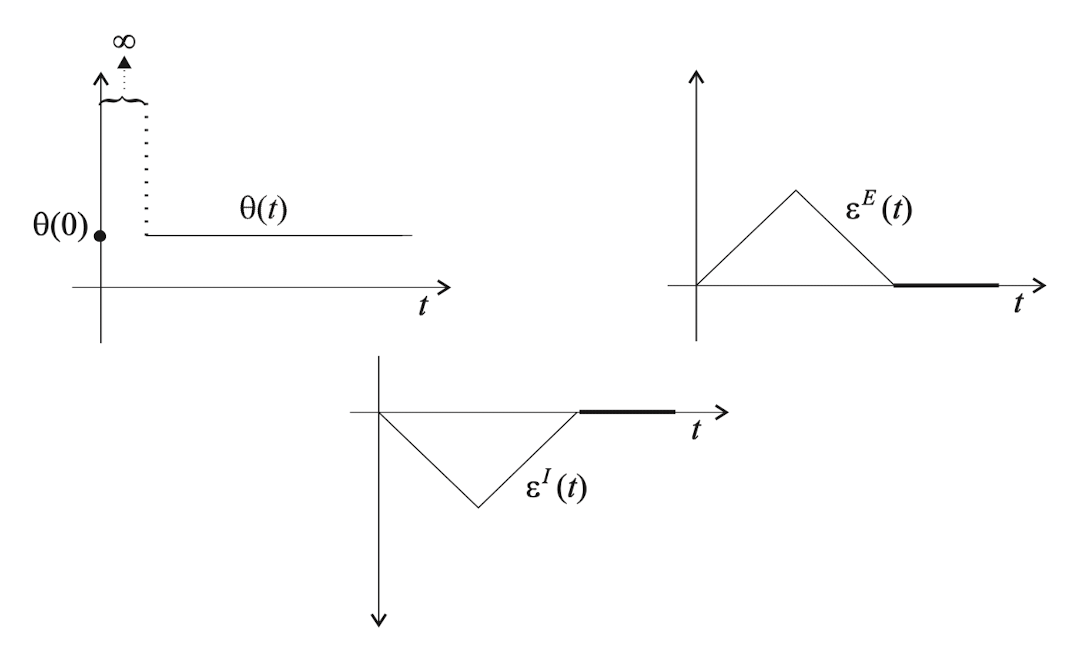
\includegraphics[width=0.5\textwidth]{response_threshold_functions.png}
    \end{center}
    \item definition of delay modules to generate arbitrary long delays during the computation, and inhibition modules that put the value of a neuron under a certain threshold $\kappa$ for at least time $\lambda$
    \item definition of oscillators that send a spike periodically, according to a period $\pi$, and with a phase $\varphi$. These oscillators allow to make step-by-step computation by synchronizing everything together, and store values as phase differences.
    \item synchronization module: sometimes an operation will be defined without caring about time synchronization with the main oscillator of the SNN. This module is put in the output of such operations, in order to re-synchronize the computation.
    \item simulation of boolean threshold circuit, in order to be able to implement the transition function of the Turing machine
    \item comparison and multiplication of phases, which are useful to compute stacks encoded as a real number
    \item simulation of a stack under the for of a real number
    \item simulation of a Turing machine: putting together all the above elements to simulate a Turing machine on the basis of phase differences
    \item weight to phase transformation: this allows to define the NN with only weights, and the translate these weights to phase differences to be able to carry the computations defined above
    \item construction of the NN: putting everything above together to define a fixed neural network that simulates universal Turing machines
 \end{enumerate}

 The author talks about going further beyond Turing machines. He explains that the SNNs correspond exactly to real-valued RAMs, which are also equivalent to to RNNs allowing heavyside functions. However, Turing completeness can be achieved without the comparison module, which basically makes everything simpler and non-Turing power.


\end{document}